\chapter{Tán xạ, đối ngẫu và biên độ Veneziano}

\lectureoverview{Tán xạ quy giản một va chạm thành những dữ liệu bất biến có thể so sánh với thực nghiệm. Đối với bốn hạt đồng nhất, những dữ liệu ấy có thể được sắp xếp thành các biến Mandelstam \(s,t,u\), trong đó chỉ có hai biến là độc lập. Khi đó, trao đổi hạt thông thường gợi ra các kênh trực tiếp và kênh chéo tách biệt. Biên độ Veneziano đã đảo lộn kỳ vọng ấy: một hàm chứa cả hai mô tả kênh. Nửa sau của bài giảng xây dựng hàm đó từ hai dây mở nhập lại, tiến hóa như một chuỗi dao động duy nhất, rồi lại tách ra.}

\section{Một lý thuyết phải dự đoán điều gì}

Dây fermion giải quyết hai khuyết điểm của mô hình thuần boson: chúng thừa nhận các trạng thái fermion và, sau phép chiếu thích hợp, loại bỏ tachyon. Số chiều không-thời gian tới hạn của chúng là 10 chứ không phải 26. Vì vậy các chiều phụ vẫn còn, nhưng việc compact hóa chúng được hoãn lại. Chủ đề trước mắt là tán xạ.
\editorialnote{Phát biểu về việc không có tachyon nói về phổ siêu dây nhất quán sau phép chiếu bắt buộc; chỉ riêng việc thêm các fermion trên mặt thế giới tự nó vẫn chưa đủ.}

Tán xạ không nhất thiết là điều thú vị nhất mà các hạt làm. Nó đơn giản là thao tác mà một thí nghiệm có thể lặp lại một cách sạch sẽ. Cho các hạt xác định lao vào nhau, ghi lại các hạt xuất hiện từ va chạm, rồi suy ra động lực học ẩn bên trong vùng tương tác. Một lý thuyết trở nên định lượng khi nó cung cấp một biên độ phức \begin{equation}
  \mathcal A(\hbox{incoming data}\to\hbox{outgoing data}),
\end{equation} mà bình phương độ lớn của nó, cùng với các hệ số không gian pha thông thường, cho xác suất của kết cục đó.

\begin{figure}[H]
  \centering
  
\includegraphics[width=0.72\textwidth]{lecture_06_figure_01.png}
  \caption{Các hạt tới đi vào một vùng tương tác hộp đen và các hạt ra xuất hiện; thời gian được vẽ theo phương ngang.}
  \lectureframe{00:02:35}
  \label{fig:l06-black-box}
\end{figure}

Các hạt còn mang spin, điện tích và nhãn loại hạt. Để trước hết làm lộ ra phần động học, ta tạm thời bỏ qua mọi thứ trừ xung lượng.

\section{Bốn-xung lượng và quy ước mọi hạt đều đi vào}

Viết bốn-xung lượng của một hạt dưới dạng
\begin{equation}
  k^\mu=(k^0,\mathbf k)=(E,\mathbf p).
\end{equation}
Bài giảng dùng metric chủ yếu-dương, nên
\begin{equation}
  k^2\equiv \mathbf p^2-E^2.
\end{equation}
Vì vậy hệ thức tán sắc tương đối tính là
\begin{equation}
  E^2-\mathbf p^2=m^2,
  \qquad
  k^2=-m^2.
  \label{eq:l06-mass-shell}
\end{equation}
Thay đổi xung lượng không gian sẽ làm thay đổi năng lượng, nhưng không đưa hạt ra khỏi vỏ khối lượng của nó.

\begin{figure}[H]
  \centering
  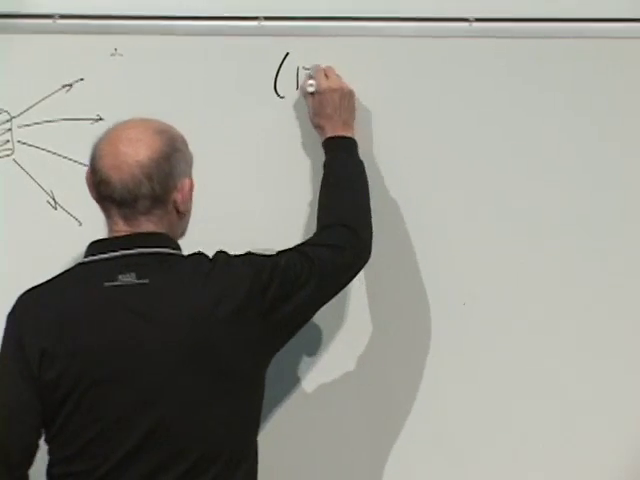
\includegraphics[width=0.66\textwidth]{lecture_06_figure_02.png}
  \caption{Điều kiện vỏ khối lượng trong quy ước metric được dùng xuyên suốt bài giảng.}
  \lectureframe{00:05:56}
  \label{fig:l06-mass-shell}
\end{figure}

Xét hai hạt đi vào với các xung lượng \(k_1,k_2\) và hai hạt đi ra với các xung lượng vật lý \(q_3,q_4\). Bảo toàn năng lượng và xung lượng là một phương trình bốn-véc-tơ,
\begin{equation}
  k_1+k_2=q_3+q_4.
  \label{eq:l06-physical-conservation}
\end{equation}
Thuận tiện hơn là gán một xung lượng đi vào cho mọi đường ngoài:
\begin{equation}
  k_3\equiv-q_3,
  \qquad
  k_4\equiv-q_4.
\end{equation}
Khi đó
\begin{equation}
  k_1+k_2+k_3+k_4=0,
  \label{eq:l06-all-incoming}
\end{equation}
và mọi chân đều thỏa \(k_i^2=-m_i^2\). Các hạt đi ra chỉ có năng lượng âm trong quy ước ghi chép này; các năng lượng vật lý của chúng vẫn dương.

\begin{figure}[H]
  \centering
  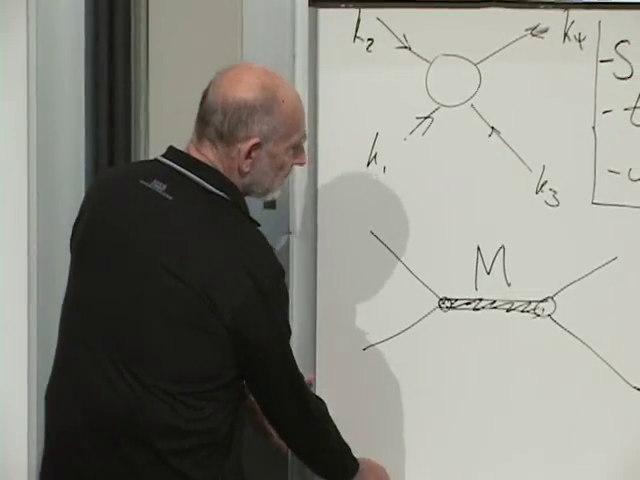
\includegraphics[width=0.68\textwidth]{lecture_06_figure_03.png}
  \caption{Các xung lượng ra vật lý được đảo dấu để cả bốn xung lượng ngoài có thể được xử lý đối xứng như các xung lượng đi vào.}
  \lectureframe{00:09:10}
  \label{fig:l06-all-incoming-board}
\end{figure}

Thoạt đầu, biên độ có vẻ là một hàm của 16 thành phần, \(\mathcal A(k_1,k_2,k_3,k_4)\). Phần lớn trong số đó là thừa. Hãy chuyển sang hệ quy chiếu tâm khối, xoay các xung lượng tới theo một trục đã chọn, và để đơn giản hãy giả sử cả bốn hạt đều có cùng khối lượng. Khi đó trạng thái tới được xác định bởi một đại lượng duy nhất, năng lượng tâm khối. Các xung lượng không gian đi ra phải bằng nhau và ngược chiều nhau, đồng thời có cùng độ lớn với cặp đi vào. Chỉ còn lại góc lệch \(\theta\) của chúng. Vì vậy quá trình có hai biến động học độc lập:
\begin{equation}
  E_{\mathrm{cm}},
  \qquad
  \theta.
  \label{eq:l06-two-data}
\end{equation}

\section{Các biến Mandelstam}

Hai đại lượng vật lý trong \eqref{eq:l06-two-data} phải có thể được biểu diễn mà không cần chọn hệ quy chiếu. Với quy ước mọi hạt đều đi vào, hãy định nghĩa
\begin{equation}
  \begin{aligned}
    -s&=(k_1+k_2)^2,\\
    -t&=(k_1+k_3)^2,\\
    -u&=(k_1+k_4)^2.
  \end{aligned}
  \label{eq:l06-mandelstam}
\end{equation}
Trong hệ tâm khối, các phần không gian của \(k_1+k_2\) triệt tiêu nhau, do đó
\begin{equation}
  s=E_{\mathrm{cm}}^2.
  \label{eq:l06-s-energy}
\end{equation}

Đối với một xung lượng vật lý đi ra \(q_3=-k_3\),
\begin{equation}
  k_1+k_3=k_1-q_3
\end{equation}
là xung lượng truyền từ chân 1 sang chân 3. Với các khối lượng ngoài bằng nhau, và độ lớn xung lượng không gian đi vào là \(p\),
\begin{equation}
  -t=2p^2(1-\cos\theta),
  \qquad
  -u=2p^2(1+\cos\theta).
  \label{eq:l06-tu-angle}
\end{equation}
Vì thế \(t\) và \(u\) mang thông tin góc mà các đầu dò đo được.

\begin{figure}[H]
  \centering
  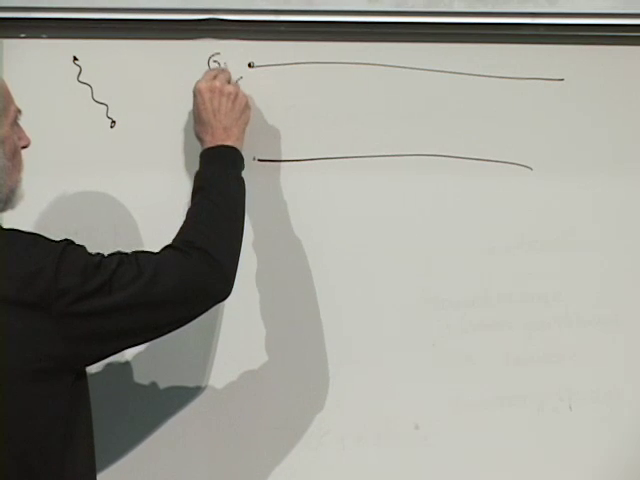
\includegraphics[width=0.74\textwidth]{lecture_06_figure_04.png}
  \caption{Các định nghĩa đối xứng của \(s,t,u\) trong quy ước mọi hạt đều đi vào.}
  \lectureframe{00:26:20}
  \label{fig:l06-stu-board}
\end{figure}

Ba ký hiệu không có nghĩa là ba dữ kiện độc lập. Bình phương \eqref{eq:l06-all-incoming} và dùng \(k_i^2=-m^2\) cho
\begin{equation}
  s+t+u=4m^2
  \label{eq:l06-stu-constraint}
\end{equation}
đối với các khối lượng bằng nhau. Một khi \(s\) và \(t\) đã biết, \(u\) được xác định.

\begin{classroomqa}
\audiencequestion{Liệu chân không có thể làm chậm một hạt chuyển động tự do, gần như ma sát, hay không? \lecturetimestamp{00:27:17}}
\lecturerresponse{Không thể trong một chân không bất biến tịnh tiến. Không có nơi nào để phần xung lượng bị thiếu hụt đi tới, nên bảo toàn xung lượng cấm kiểu ma sát như vậy. Người ta có thể hình dung một môi trường hoặc một chân không khác chọn ra một hệ quy chiếu nghỉ ưu tiên, nhưng đó không phải là chân không đang được dùng ở đây.}
\end{classroomqa}

\begin{classroomqa}
\audiencequestion{Vì sao hai hạt đi ra nhất thiết phải có năng lượng bằng nhau? \lecturetimestamp{00:27:54}}
\lecturerresponse{Trong hệ tâm khối, các xung lượng không gian của chúng phải bằng nhau và ngược chiều nhau. Đối với quá trình khối lượng bằng nhau đang bàn tới, độ lớn xung lượng bằng nhau kéo theo năng lượng bằng nhau theo \(E^2=p^2+m^2\). Nếu các khối lượng đi ra khác nhau, kết luận cuối cùng ấy sẽ phải được sửa đổi.}
\end{classroomqa}

\section{Các kênh trực tiếp và chéo}

Một sơ đồ hạt điểm đơn giản cho phép các hạt 1 và 2 tạo thành một hạt trung gian có khối lượng \(M\), rồi hạt đó phân rã thành 3 và 4. Bỏ qua các thừa số ở tử số và quy tắc cực, sự phụ thuộc đặc trưng của nó là
\begin{equation}
  \mathcal A_s\sim\frac{g^2}{s-M^2}.
  \label{eq:l06-s-channel}
\end{equation}
Đây là quá trình trực tiếp, hay quá trình kênh \(s\). Xoay cách nối sang ngang cho ta sự trao đổi giữa hai đường ngoài,
\begin{equation}
  \mathcal A_t\sim\frac{g^2}{t-M^2},
  \label{eq:l06-t-channel}
\end{equation}
đó là quá trình chéo, hay quá trình kênh \(t\). Một cách nối thứ ba cho
\begin{equation}
  \mathcal A_u\sim\frac{g^2}{u-M^2}.
  \label{eq:l06-u-channel}
\end{equation}

\begin{figure}[H]
  \centering
  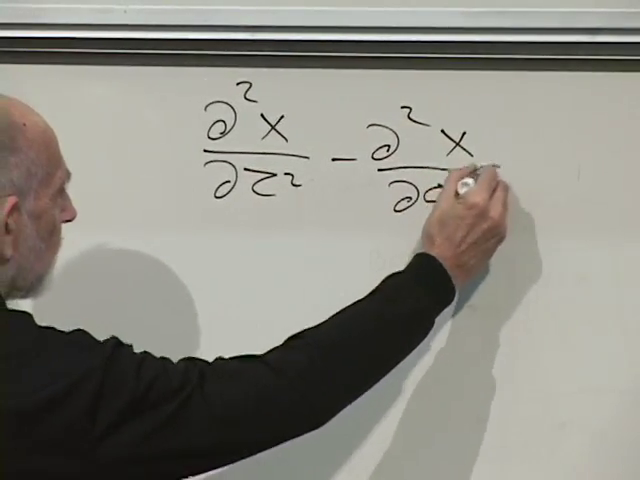
\includegraphics[width=0.72\textwidth]{lecture_06_figure_05.png}
  \caption{Sự tạo thành trực tiếp qua một trạng thái trung gian và cực tương ứng \(g^2/(s-M^2)\); cách nối chéo đang được dựng trên cùng một bảng.}
  \lectureframe{00:30:50}
  \label{fig:l06-channel-board}
\end{figure}

Sự phân biệt này là vật lý. Ở mức vô hướng thô sơ này, \eqref{eq:l06-s-channel} phụ thuộc vào năng lượng va chạm nhưng không phụ thuộc vào góc. Trạng thái hợp thành đã quên hướng tới ban đầu trước khi phân rã, nên sự phân rã của nó là đẳng hướng. Biên độ trao đổi phụ thuộc vào xung lượng truyền và vì thế phụ thuộc vào góc; một hạt trao đổi nhẹ rất thiên về độ lệch nhỏ. Spin sẽ còn bổ sung thêm phụ thuộc góc nữa, nhưng cấu trúc cực đã hiện rõ.

\begin{classroomqa}
\audiencequestion{Kênh \(u\) còn thiếu có sinh ra một hạng thứ ba không? \lecturetimestamp{00:34:47}}
\lecturerresponse{Có, bất cứ khi nào các bản sắc hạt và các ghép nối cho phép cách nối đó. Khi ấy ta thêm một hạng có cực tại \(u=M^2\). Nó không phải là một biến động học độc lập mới, vì \(s+t+u=4m^2\), nhưng nó là một sơ đồ kênh riêng biệt.}
\end{classroomqa}

\section{Một hàm, hai mô tả kênh}

Một cực đơn là một mô hình nghèo nàn của tán xạ meson. Hai meson có thể tạo thành nhiều cộng hưởng, với một tháp các khối lượng và mômen góc. Phản ứng đầu tiên vào những năm 1960 là thêm nhiều cực kênh \(s\) hơn, nhiều cực kênh \(t\) hơn, và các cực kênh \(u\) được phép. Sau đó người ta tìm được một hàm kinh tế hơn nhiều. Trong đơn vị của bài giảng, nơi quỹ đạo Regge tuyến tính và hệ số chặn của nó đã được hấp thụ vào \(s\) và \(t\), hàm đó là
\begin{equation}
  \mathcal A_{\mathrm V}(s,t)
  \propto
  \frac{\Gamma(-s)\Gamma(-t)}{\Gamma(-s-t)}.
  \label{eq:l06-veneziano}
\end{equation}
Hàm gamma mở rộng giai thừa:
\begin{equation}
  \Gamma(n)=(n-1)!
\end{equation}
ở các số nguyên dương.

\begin{figure}[H]
  \centering
  \includegraphics[width=0.68\textwidth]{lecture_06_figure_06.png}
  \caption{Biên độ Veneziano được viết như một tỉ số đối xứng của các hàm gamma.}
  \lectureframe{00:42:25}
  \label{fig:l06-veneziano-board}
\end{figure}

Các cực của \(\Gamma(-s)\) tái tạo một tháp vô hạn các cộng hưởng kênh trực tiếp. Tuy vậy, chính biểu thức ấy lại đối xứng dưới \(s\leftrightarrow
t\), nên các cực \(\Gamma(-t)\) của nó cho một khai triển theo kênh chéo. Đây không phải là hai đóng góp được cộng vào một cách riêng rẽ. Một hàm giải tích duy nhất chấp nhận một trong hai mô tả. Đó là ý tưởng cổ điển về đối ngẫu giữa các cộng hưởng kênh trực tiếp và các trao đổi kênh chéo.

\begin{classroomqa}
\audiencequestion{Làm sao một biên độ có thể chứa cả hai tổng theo kênh mà không cần cộng chúng lại? \lecturetimestamp{00:43:32}}
\lecturerresponse{Chính đó mới là điều bất ngờ. Khai triển hàm gần các cực kênh \(s\) của nó sẽ tổ chức nó thành các cộng hưởng trực tiếp; khai triển gần các cực kênh \(t\) của nó sẽ tổ chức chính hàm ấy thành các trao đổi. Cần có một mô hình vi mô để giải thích vì sao hai cách đọc đó lại là một, và mô hình ấy là một dây tương tác.}
\end{classroomqa}

\section{Một dải do một dây mở quét ra}

Tham số hóa một dây mở bằng
\begin{equation}
  0\leq\sigma\leq\pi.
\end{equation}
Nhãn \(\sigma\) không phải là một vị trí trong không-thời gian. Phép nhúng \(X^\mu(\sigma,\tau)\) cho ta biết điểm mang nhãn đó nằm ở đâu trong không-thời gian, còn \(\tau\) đo sự tiến hóa. Một hạt điểm quét ra một đường thế giới; dây đang chuyển động quét ra một mặt thế giới hai chiều. Trong lý thuyết tự do, mỗi tọa độ nhúng đều thỏa
\begin{equation}
  \frac{\partial^2X^\mu}{\partial\tau^2}
  -
  \frac{\partial^2X^\mu}{\partial\sigma^2}
  =0.
  \label{eq:l06-wave-equation}
\end{equation}

\begin{figure}[H]
  \centering
  \includegraphics[width=0.70\textwidth]{lecture_06_figure_07.png}
  \caption{Phương trình sóng chi phối mỗi tọa độ của dây tự do trên dải mặt thế giới.}
  \lectureframe{00:49:10}
  \label{fig:l06-wave-equation-board}
\end{figure}

Đối với việc xây dựng tán xạ, sẽ có ích nếu chưa vội lấy giới hạn liên tục. Hãy thay mỗi dây bằng \(n\) điểm khối lượng nối với nhau bằng các lò xo. Mặt thế giới trở thành một tập dày đặc các đường thế giới kề nhau, và các mode chuẩn của nó là các dao động tử điều hòa thông thường. Hai chuỗi tới có thể chạm nhau ở các đầu mút. Tại biến cố ấy, một lò xo mới nối chúng lại, chúng tiến hóa trong một khoảng \(\tau\) như một chuỗi dài hơn duy nhất, rồi về sau một lò xo đứt ra để hai chuỗi đi ra xuất hiện.

\begin{figure}[H]
  \centering
  \includegraphics[width=0.72\textwidth]{lecture_06_figure_08.png}
  \medskip

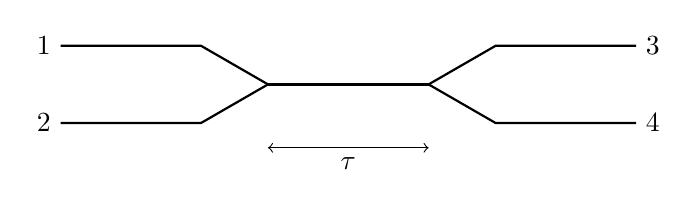
\begin{tikzpicture}[x=0.85cm,y=0.70cm]
    \draw[thick] (0,2.2) -- (2.1,2.2) -- (3.1,1.5);
    \draw[thick] (0,0.8) -- (2.1,0.8) -- (3.1,1.5);
    \draw[thick] (3.1,1.5) -- (5.5,1.5);
    \draw[thick] (5.5,1.5) -- (6.5,2.2) -- (8.6,2.2);
    \draw[thick] (5.5,1.5) -- (6.5,0.8) -- (8.6,0.8);
    \draw[<->] (3.1,0.35) -- node[below] {\(\tau\)} (5.5,0.35);
    \node[left] at (0,2.2) {1};
    \node[left] at (0,0.8) {2};
    \node[right] at (8.6,2.2) {3};
    \node[right] at (8.6,0.8) {4};
  \end{tikzpicture}
  \caption{Hai dây mở được rời rạc hóa chạm nhau, tạo thành một dây trung gian trong khoảng \(\tau\), rồi tách ra. Khung hình gốc giữ nguyên cấu trúc lò xo và đường thế giới; hình sơ đồ tách riêng cách nối của nó.}
  \lectureframe{00:51:25}
  \label{fig:l06-string-joining}
\end{figure}

Hai dây chỉ được vẽ kề nhau trong không gian tham số. Các vị trí của chúng trong không-thời gian không nhất thiết phải kề nhau cho đến khi các tọa độ đầu mút thực sự trùng nhau. Tự do tái tham số hóa cho phép đặt các biến cố nối và tách tại những vị trí thuận tiện trên hình; sự tự do hình học này sẽ trở thành đối xứng bảo giác trong bài giảng tiếp theo.

\section{Phép tính dao động tử từng bước}

Gọi các tọa độ của chuỗi thứ nhất là \(x_1,\ldots,x_n\), và của chuỗi thứ hai là \(x_{n+1},\ldots,x_{2n}\). Tọa độ tâm khối của chúng là
\begin{equation}
  X_{\mathrm{cm}}^{(1)}
  =\frac1n\sum_{a=1}^{n}x_a,
  \qquad
  X_{\mathrm{cm}}^{(2)}
  =\frac1n\sum_{a=n+1}^{2n}x_a.
  \label{eq:l06-chain-centers}
\end{equation}
Một chuỗi có xung lượng xác định \(k_1\) có một sóng phẳng tâm khối nhân với một trạng thái cơ bản dao động tử nội tại:
\begin{align}
  \Psi_1
  &=
  e^{ik_1\cdot X_{\mathrm{cm}}^{(1)}}
  \psi_0(x_1,\ldots,x_n),
  \\
  \Psi_2
  &=
  e^{ik_2\cdot X_{\mathrm{cm}}^{(2)}}
  \psi_0(x_{n+1},\ldots,x_{2n}).
  \label{eq:l06-two-wavefunctions}
\end{align}
Các thừa số \(\psi_0\) phụ thuộc vào các tọa độ tương đối, chứ không phụ thuộc vào phép tịnh tiến chung của cả chuỗi. Vì các dây tới lúc đầu là những hệ lượng tử tách biệt,
\begin{equation}
  \Psi_{\mathrm{in}}=\Psi_1\Psi_2.
  \label{eq:l06-product-state}
\end{equation}

\begin{figure}[H]
  \centering
  \includegraphics[width=0.76\textwidth]{lecture_06_figure_09.png}
  \caption{Hai sóng phẳng xung lượng và các thừa số trạng thái cơ bản dao động tử nội tại của chúng, được viết bằng các màu khác nhau.}
  \lectureframe{00:58:05}
  \label{fig:l06-wavefunctions-board}
\end{figure}

Sự nối chọn ra phần của hàm sóng này mà tại đó hai tọa độ đầu mút trùng nhau:
\begin{equation}
  x_n=x_{n+1}.
  \label{eq:l06-endpoint-contact}
\end{equation}
Ở thời điểm đó, các tọa độ khác không đổi. Trạng thái được chọn sau đó được cho tiến hóa bằng Hamiltonian \(H_{\mathrm{joined}}\) của chuỗi dài hơn duy nhất:
\begin{equation}
  \Psi(\tau)
  =
  e^{-iH_{\mathrm{joined}}\tau}\Psi(0).
  \label{eq:l06-time-evolution}
\end{equation}
Cuối cùng, ta lấy độ chồng lấp của nó với tích các trạng thái dây đi ra mang xung lượng \(q_3,q_4\).

\begin{figure}[H]
  \centering
  \includegraphics[width=0.76\textwidth]{lecture_06_figure_10.png}
  \caption{Hàm sóng hai chuỗi ngay trước khi điều kiện trùng nhau của các đầu mút được áp đặt.}
  \lectureframe{00:58:55}
  \label{fig:l06-endpoint-board}
\end{figure}

Phép tính thì dài nhưng không bí hiểm. Mỗi tọa độ nội tại đều có thể được phân rã thành các mode dao động tử, nên độ chồng lấp khi nối, sự tiến hóa theo thời gian và phép chiếu cuối cùng đều quy về đại số Gaussian của các dao động tử. Điều còn chưa được cố định là thời gian sống \(\tau\) của dây đã nối.

\begin{classroomqa}
\audiencequestion{Các hàm sóng màu đen và đỏ được cộng hay nhân với nhau? \lecturetimestamp{01:02:26}}
\lecturerresponse{Nhân. Trạng thái tích tensor của hai hệ độc lập được biểu diễn trong cơ sở tọa độ bằng tích các hàm sóng của chúng. Phép cộng sẽ mô tả một chồng chập của các khả năng, chứ không phải sự hiện diện đồng thời của cả hai dây đi vào.}
\end{classroomqa}

\begin{classroomqa}
\audiencequestion{Tại sao lại lấy tích phân theo thời gian trung gian
\(\tau\)? \lecturetimestamp{01:04:04}}
\lecturerresponse{Không gán cho dây đã nối một thời gian sống cố định.
Quy tắc của Feynman là cộng các biên độ trên mọi lịch sử được phép. Trong mô tả này, tham số lịch sử liên tục còn lại là thời gian giữa lúc nối và lúc tách, nên tổng trở thành một tích phân trên
\(0\leq\tau<\infty\).}
\end{classroomqa}

\section{Từ thời gian truyền đến hàm beta}

Sau khi tính các độ chồng lấp của các dao động tử, kết quả có thể được sắp xếp thành
\begin{equation}
  \mathcal A(s,t)
  \propto
  \int_0^\infty d\tau\,
  e^{\tau(s+1)}
  \bigl(1-e^{-\tau}\bigr)^{-t-1}
  e^{-\tau}.
  \label{eq:l06-tau-integral}
\end{equation}
Thừa số \(e^{-\tau}\) ở cuối được giữ tường minh vì đó là nhân tử Jacobi cần cho bước tiếp theo. Tương đương, các hàm mũ thứ nhất và cuối cùng kết hợp thành
\(e^{s\tau}\).

\begin{figure}[H]
  \centering
  \includegraphics[width=0.76\textwidth]{lecture_06_figure_11.png}
  \caption{Biểu thức dưới dấu tích phân theo thời gian truyền sau phép tính dao động tử;
  thừa số \(e^{-\tau}\) tách riêng cung cấp nhân tử Jacobi
  cho phép đổi biến.}
  \lectureframe{01:06:45}
  \label{fig:l06-tau-integral-board}
\end{figure}

Bây giờ đặt
\begin{equation}
  z=e^{-\tau},
  \qquad
  dz=-e^{-\tau}\,d\tau.
  \label{eq:l06-z-substitution}
\end{equation}
Khi \(\tau\) chạy từ \(0\) đến \(\infty\), \(z\) chạy từ \(1\) đến \(0\).
Dấu trừ đảo ngược các cận, do đó thu được
\begin{equation}
  \mathcal A(s,t)
  \propto
  \int_0^1
  z^{-s-1}(1-z)^{-t-1}\,dz.
  \label{eq:l06-beta-integral}
\end{equation}

\begin{figure}[H]
  \centering
  \includegraphics[width=0.74\textwidth]{lecture_06_figure_12.png}
  \caption{Phép thế \(z=e^{-\tau}\) làm lộ ra tích phân beta
  Euler.}
  \lectureframe{01:08:49}
  \label{fig:l06-beta-integral-board}
\end{figure}

Tích phân này được xác định trực tiếp trong miền mà nó hội tụ tại các đầu mút, và ở những miền khác thì bằng phép tiếp tục giải tích. Nó chính là hàm beta Euler:
\begin{equation}
  B(-s,-t)
  =
  \frac{\Gamma(-s)\Gamma(-t)}{\Gamma(-s-t)}.
  \label{eq:l06-beta-gamma}
\end{equation}

\begin{figure}[H]
  \centering
  \includegraphics[width=0.72\textwidth]{lecture_06_figure_13.png}
  \caption{Trên bảng, tích phân đã biến đổi được đồng nhất với
  \(B(-s,-t)\) và bắt đầu được viết lại về dạng hàm gamma của nó.}
  \lectureframe{01:12:24}
  \label{fig:l06-beta-gamma-board}
\end{figure}

Đối xứng kênh giờ đây trở nên hiển nhiên. Dưới phép biến đổi \(z\mapsto1-z\),
\begin{equation}
  \int_0^1 z^{-s-1}(1-z)^{-t-1}\,dz
  =
  \int_0^1 z^{-t-1}(1-z)^{-s-1}\,dz.
\end{equation}
Vì thế \(\mathcal A(s,t)=\mathcal A(t,s)\). Một quá trình được xây dựng như hai dây nối lại rồi sau đó tách ra tự động cũng chứa mô tả kênh chéo.
\editorialnote{Bài giảng lược bỏ độ dốc Regge và hệ số chặn trong các đối số của hàm beta. Trong ký hiệu chuẩn, người ta thay \(s,t\)
bằng các quỹ đạo tuyến tính tương ứng \(\alpha(s),\alpha(t)\). Tính đối ngẫu và lập luận đổi biến không thay đổi.}

\begin{classroomqa}
\audiencequestion{Tỷ số các hàm gamma trông giống những biểu thức
giai thừa trong tổ hợp học. Có một cách diễn giải đếm trực tiếp
về mặt vật lý nào không? \lecturetimestamp{01:13:22}}
\lecturerresponse{Với các đối số nguyên, hàm beta liên hệ với một
tỷ số như \(n!\,m!/(n+m)!\), nhưng ở đây không hề khẳng định có một
cơ chế tổ hợp nào. Cùng một hàm đặc biệt đó cũng xuất hiện từ tích phân
trên mặt thế giới; sự giống nhau này không phải là con đường đã dẫn tới việc tìm ra
biên độ.}
\end{classroomqa}

Lý do còn chưa lộ ra khiến một mặt thế giới có thể được diễn giải theo cả hai kênh là đối xứng bảo giác. Nó cho phép mặt ấy bị kéo giãn như kẹo kéo mà không làm thay đổi biên độ, biến một vùng truyền dài của kênh trực tiếp thành một bức tranh trao đổi ở kênh chéo. Cách giải thích hình học đó được dời sang bài giảng tiếp theo.

\section{Phép kiểm tra tán xạ đã xác lập điều gì}
\enlargethispage{3\baselineskip}
\begingroup
\setlength{\medskipamount}{3pt plus 1pt minus 1pt}

Bức tranh nối rời rạc đã gợi ra một loạt câu hỏi cuối cùng.

\begin{classroomqa}
\audiencequestion{Nếu hai chuỗi, mỗi chuỗi gồm \(n\) thành phần, nối nhau tại các
đầu mút, thì kết quả có phải là \(2n-1\) không, và điều đó có thể làm thay đổi chẵn lẻ
fermion không? \lecturetimestamp{01:16:16}}
\lecturerresponse{Trong bức tranh hadron ở đầu mút, cặp đầu mút tiếp xúc
có thể được xem như một cặp hạt-phản hạt hủy nhau, nên
số đếm giảm đi hai chứ không phải một. Trong giới hạn liên tục, sai khác hữu hạn giữa \(2n\) và \(2n-2\) là không quan trọng, nhưng việc bảo toàn chẵn lẻ fermion
thì không phải vậy. Các thành phần trên mạng chỉ là một bộ điều chuẩn cho
dây liên tục, chứ không phải những hạt cườm cơ bản theo nghĩa đen.}
\end{classroomqa}

\begin{classroomqa}
\audiencequestion{Phần thảo luận về sau có đi tiếp vào toàn bộ
toán học của siêu dây không? \lecturetimestamp{01:18:05}}
\lecturerresponse{Chỉ một số hệ quả chọn lọc sẽ được dùng. Lộ trình trước mắt
đi qua đối xứng mặt thế giới và compact hóa, tiếp theo là một
điểm xuất phát khác được phát triển vào giữa thập niên 1990: M-lý thuyết. Mục đích
của nó là đi tới cùng một vật lý từ một quan điểm trong đó một số đặc điểm vốn dĩ
phức tạp trở nên minh bạch.}
\end{classroomqa}

\begin{classroomqa}
\audiencequestion{Quy tắc nối này chỉ là một gợi ý từ các va chạm
meson thôi sao? \lecturetimestamp{01:20:02}}
\lecturerresponse{Tán xạ meson cung cấp gợi ý về mặt lịch sử, nhưng
quy tắc này là tổng quát đối với dây hở. Cùng một tôpô mô tả các va chạm của
photon của dây hở và các trạng thái dây hở khác. Hai dây kín nối lại
rồi tách ra bằng một cách xây dựng tương tự, với một dây kín ở vùng
trung gian.}
\end{classroomqa}

\begin{classroomqa}
\audiencequestion{Phép tính này chỉ áp dụng khi các trạng thái dây là
fermion thôi sao? \lecturetimestamp{01:20:56}}
\lecturerresponse{Không. Phép tính Veneziano ban đầu thuộc về
dây hở boson. Siêu dây đòi hỏi thêm các bậc tự do fermion và
làm thay đổi chi tiết của biểu thức dưới dấu tích phân, nhưng logic về sự nối, sự truyền,
phép chiếu và đối ngẫu mặt thế giới vẫn gần như tương tự.}
\end{classroomqa}

Việc tìm thấy một trạng thái spin một hay spin hai trong phổ dao động tử là gợi ý, nhưng chưa có tính quyết định. Biên độ tán xạ của chúng mới cung cấp phép kiểm tra mạnh hơn. Các biên độ photon tuân theo những đồng nhất thức gắn với bảo toàn điện tích và bất biến chuẩn; các biên độ graviton tuân theo những ràng buộc tương ứng của một trường spin hai không khối lượng. Các trạng thái dây đã vượt qua những phép kiểm tra này trong tương tác với các trạng thái có khối lượng, các trạng thái không khối lượng, và với nhau.
Đó là lý do vì sao các nhãn photon và graviton trở thành những nhận diện vật lý chứ không phải những phỏng đoán chỉ dựa trên việc đếm phân cực.
\editorialnote{Theo ngôn ngữ hiện đại, các phép kiểm tra này được mã hóa trong sự tách rời của các phân cực phi vật lý, các đồng nhất thức Ward chuẩn, và sự ghép nối năng lượng thấp phổ quát của trạng thái spin hai không khối lượng.}

\begin{classroomqa}
\audiencequestion{Bản thân điện tích phát sinh từ đâu trong mô tả
dây? \lecturetimestamp{01:24:03}}
\lecturerresponse{Câu hỏi đó được để ngỏ ở cuối bài giảng. Câu
trả lời cho nó đòi hỏi cấu trúc nội tại và cấu trúc đầu mút của lý thuyết dây,
những điều vẫn chưa được giới thiệu, nên nó thuộc về phần thảo luận tiếp theo chứ không thuộc phép suy dẫn tán xạ này.}
\end{classroomqa}
\endgroup
